\documentclass[11pt]{article}
\usepackage[margin=1in]{geometry}
\usepackage{amsmath,amssymb,amsthm}
\usepackage{times}
\usepackage{tikz}
\usetikzlibrary{arrows.meta,positioning}
\usepackage{booktabs}
\usepackage[colorlinks=true,linkcolor=blue,citecolor=blue,urlcolor=blue]{hyperref}

% Theorem environments
\newtheorem{theorem}{Theorem}
\newtheorem{lemma}[theorem]{Lemma}
\newtheorem{proposition}[theorem]{Proposition}
\newtheorem{corollary}[theorem]{Corollary}
\theoremstyle{definition}
\newtheorem{definition}{Definition}

% Macros (kept minimal and classical)
\newcommand{\J}{J}
\newcommand{\C}{\mathcal{C}}
\newcommand{\TauZero}{\tau_{0}}
\newcommand{\phiG}{\varphi}

\title{The Minimal Complexity Functional: A Parameter\,\mbox{\textendash}\,Free Variational Principle for Physics}

\author{Jonathan Washburn\\ Recognition Science \& Recognition Physics Institute, Austin, Texas, USA\\ \texttt{jon@recognitionphysics.org}}

\date{\today}

\begin{document}

\maketitle

\begin{abstract}
We formulate a minimal\,\mbox{\textendash}\,complexity principle for physical evolution built on a single convex, symmetric, normalized functional on the positive reals,
\(\J(x)=\tfrac12(x+1/x)-1\). In logarithmic coordinates this reads \(\J(e^{t})=\cosh t-1\).
We make the hypotheses used throughout explicit and uniform: inversion symmetry \(\J(x)=\J(1/x)\); strict convexity on \(\mathbb{R}_{>0}\); calibration \(\J(1)=0\), \(\J''(1)=1\); a holomorphic extension of \(\J\) to \(\mathbb{C}\setminus\{0\}\); and at\,\mbox{\textendash}\,most\,linear growth \(\J(x)=O(x+1/x)\) as \(x\to\infty\) and \(x\to 0^{+}\).
Under these conditions one obtains uniqueness in two equivalent ways: (i) a classical d'Alembert\,\mbox{\textendash}\,type characterization in log coordinates selects \(\cosh t-1\); (ii) a Laurent\,\mbox{\textendash}\,series argument on \(\mathbb{C}\setminus\{0\}\) shows that linear growth kills all modes beyond \(x^{\pm1}\), and the calibration fixes the remaining coefficients to \(\tfrac12\) and \(-1\).
From this minimal object follow a cascade of consequences: a golden fixed point \(\phiG\) for scale recursion, a discrete eight\,\mbox{\textendash}\,tick cadence in three spatial dimensions, and a local Euler\,\mbox{\textendash}\,Lagrange equivalence that recovers stationary\,\mbox{\textendash}\,action mechanics in the quadratic regime. The Legendre dual explains the effectiveness of the Hamiltonian as an approximation. Factoring through a units\,\mbox{\textendash}\,quotient yields dimensionless identities that anchor the classical displays of \(c\), \(\hbar\), \(G\) and the fine\,\mbox{\textendash}\,structure constant without adjustable parameters. We emphasize sharp falsifiers (any alternate convex symmetric \(\J\); failure of the eight\,\mbox{\textendash}\,tick cadence; broken dimensionless identities) and an audit protocol using SI values only. The result is a parameter\,\mbox{\textendash}\,free variational foundation that unifies microscopic weights, near\,\mbox{\textendash}\,equilibrium mechanics, and large\,\mbox{\textendash}\,scale identities in a single functional.
\end{abstract}

\section{Introduction}

For more than a century, variational principles have provided a unifying language for physics. In practice, however, one usually starts by postulating an energy or action density and then fits free parameters to data. This paper pursues the opposite strategy: we show that a single, structurally\,\mbox{\textendash}\,determined functional \(\J\) on the positive reals suffices to generate the familiar variational machinery locally, while also fixing a set of dimensionless identities that eliminate adjustable knobs. The guiding requirement is minimal complexity: the functional should be uniquely selected by symmetry, normalization, and convexity, without introducing extra structure.

The central object is
\begin{equation}
  \J(x)\;=\;\tfrac12\bigl(x+x^{-1}\bigr)-1\qquad (x>0),
\end{equation}
the unique convex, symmetric functional satisfying the reciprocity symmetry \(\J(x)=\J(x^{-1})\), the local scale conditions \(\J(1)=0\), \(\J''(1)=1\), and mild regularity compatible with discrete conservation. In logarithmic coordinates \(G(t):=\J(e^{t})\), these hypotheses reduce to a classical d'Alembert\,\mbox{\textendash}\,type functional equation whose even, continuous, calibrated solution is \(G(t)=\cosh t-1\). Thus the functional is not chosen: it is forced.

From this single ingredient, several consequences follow.
First, the scale recursion induced by \(\J\) possesses a unique positive fixed point \(\phiG\) solving \(\phiG^{2}=\phiG+1\). This fixed point governs geometric ladders and quantized ratios that appear repeatedly across microphysical and emergent descriptions.
Second, when recognition or transport occurs on a discrete ledger of binary constraints, there exists a minimal neutral window whose length in three spatial dimensions is eight ticks. This eight\,\mbox{\textendash}\,tick cadence is the shortest period that covers all binary axes without timestamp multiplicity; it implies a fundamental tick \(\TauZero\) and supports a clean units\,\mbox{\textendash}\,quotient view of displays.
Third, in the quadratic neighborhood of equilibrium, write \(x=e^{\varepsilon}\) with \(|\varepsilon|\ll 1\). Then \(\J(e^{\varepsilon})=\cosh\varepsilon-1=\tfrac12\varepsilon^{2}+O(\varepsilon^{4})\), so the path action \(\C[\gamma]=\int \J(r(t))\,dt\) yields the Euler\,\mbox{\textendash}\,Lagrange equations in the usual way. A Legendre transform supplies a co\,\mbox{\textendash}\,state and an effective Hamiltonian that accurately approximates dynamics whenever deviations remain small. This explains the empirical success of energy\,\mbox{\textendash}\,based mechanics without elevating energy to a fundamental axiom.

The units\,\mbox{\textendash}\,quotient perspective is essential. Because \(\J\) fixes only dimensionless content, classical numerical displays should factor through ratios whose values are invariant under admissible rescalings. When so expressed, a small set of identities---for example, a speed identity tying a length step to a time tick, a coherence identity linking \(\hbar\) to a timescale, and a Planck\,\mbox{\textendash}\,side normalization relating length, speed, \(\hbar\), and \(G\)---can be enforced simultaneously. With the structural fixed point \(\phiG\) and the eight\,\mbox{\textendash}\,tick cadence in hand, these identities determine the classical displays of \(c\), \(\hbar\), \(G\), and the fine\,\mbox{\textendash}\,structure constant within measurement uncertainty, without introducing free parameters. In this sense, the minimal\,\mbox{\textendash}\,complexity functional closes the parameter budget.

Equally important are falsifiers and audits. The proposal fails if there exists any alternate convex symmetric \(\J\) satisfying the stated structural conditions; if the eight\,\mbox{\textendash}\,tick minimal cadence does not hold under the neutrality constraints; or if the dimensionless identities are violated beyond combined experimental uncertainty. Audits should therefore compare only invariant ratios and enforce identity closure along dual routes (e.g., time\,\mbox{\textendash}\,first versus length\,\mbox{\textendash}\,first constructions), never introducing medium\,\mbox{\textendash}\,dependent knobs.

Contributions of this paper are as follows:
\begin{itemize}
  \item We state a minimal, classical hypothesis set under which \(\J(x)=\tfrac12(x+1/x)-1\) is the unique admissible functional on \(\mathbb{R}_{>0}\).
  \item We show how \(\J\) yields (i) a golden fixed point \(\phiG\), (ii) an eight\,\mbox{\textendash}\,tick minimal cadence in three dimensions, and (iii) a local Euler\,\mbox{\textendash}\,Lagrange equivalence with a Legendre\,\mbox{\textendash}\,dual Hamiltonian.
  \item We formulate an invariants\,\mbox{\textendash}\,only audit of core identities that pins classical displays without adjustable parameters, together with clear falsifiers.
\end{itemize}

The remainder of the manuscript develops these points in classical notation: Section~2 states the axioms and proves uniqueness in log coordinates; Section~3 derives the structural consequences (\(\phiG\), eight\,\mbox{\textendash}\,tick, neutral windows); Section~4 establishes the local variational equivalence and Hamiltonian bridge; Section~5 presents identity closures and an audit protocol; Section~6 outlines predictions, tests, and falsifiers.

\section{The minimal\,\mbox{\textendash}\,complexity functional}

\paragraph{Axioms.}
\begin{definition}[Axioms for the minimal complexity functional]
We consider a functional \(\J: \mathbb{R}_{>0} \to \mathbb{R}\) subject to the following uniform structural requirements:
\begin{itemize}
  \item \textbf{Symmetry (reciprocity).} \(\J(x) = \J(x^{-1})\) for all \(x>0\).
  \item \textbf{Normalization (local scale fixing).} \(\J(1)=0\) and \(\J''(1)=1\).
  \item \textbf{Strict convexity.} \(\J\) is strictly convex on \(\mathbb{R}_{>0}\).
  \item \textbf{Analyticity.} \(\J\) is real\,\mbox{\textendash}\,analytic on \(\mathbb{R}_{>0}\) and extends holomorphically to \(\mathbb{C}\setminus\{0\}\); the inversion symmetry extends to this domain.
  \item \textbf{Linearity at the ends.} \(\J(x)=O(x+1/x)\) as \(x\to\infty\) and as \(x\to 0^{+}\).
  \item \textbf{Averaging on the exponential axis.} Writing \(G(t):=\J(e^{t})\) and \(F(t):=G(t)+1\), assume for all \(t,u\in\mathbb{R}\)
  \[
    \frac{F(t+u)+F(t-u)}{2} = F(t)\,F(u)\,.
  \]
  This encodes two\,\mbox{\textendash}\,sided averaging along \(x=e^{t}\) and, with evenness and calibration, yields the d'Alembert characterization of \(\cosh\).
\end{itemize}
\end{definition}
Either the analyticity\,+\,growth route (Laurent view) or the exp\,\mbox{\textendash}\,axis averaging route (functional equation) suffices to force uniqueness; we present both.

\begin{theorem}[Uniqueness of the minimal complexity functional]\label{thm:uniqueJ}
Under the axioms above, the unique admissible functional on \(\mathbb{R}_{>0}\) is
\(\displaystyle \J(x)=\tfrac12(x+x^{-1})-1\).
\end{theorem}
\noindent\emph{Proof sketch.} \emph{(Functional equation)} With \(G(t)=\J(e^{t})\) and \(F=G+1\), the averaging axiom gives \(F(t+u)+F(t-u)=2F(t)F(u)\). By evenness, continuity, \(F(0)=1\), \(F''(0)=1\), the standard solution is \(F(t)=\cosh t\), hence \(\J(e^{t})=\cosh t-1\). \emph{(Laurent)} Analyticity on \(\mathbb{C}\setminus\{0\}\) and inversion symmetry force a symmetric Laurent expansion \(\J(z)=a_0+\sum_{n\ge1}a_n(z^{n}+z^{-n})\). Linearity at the ends kills all \(n\ge 2\); normalization and \(\J''(1)=1\) fix \(a_1=\tfrac12\), \(a_0=-1\). Restricting to \(z=x>0\) gives the claim. \qed

\paragraph{Uniqueness (log view).}
Define the logarithmic reparametrization \(G:\mathbb{R}\to\mathbb{R}\) by \(G(t):=\J(e^{t})\). The reciprocity symmetry makes \(G\) even, \(G(-t)=G(t)\); normalization enforces \(G(0)=0\) and \(G''(0)=1\); continuity and convexity transfer to \(G\). A classical d'Alembert\,\mbox{\textendash}\,type identity characterizes \(G\):
\begin{equation}\label{eq:cosh-add}
  G(t+u) + G(t-u) \;=\; 2\,\big(G(t)\,G(u)\big) + 2\,\big(G(t)+G(u)\big)\qquad (t,u\in\mathbb{R}).
\end{equation}
\begin{lemma}[Even d'Alembert solutions]\label{lem:dA}
If \(F\) is continuous, even, \(F(0)=1\), and satisfies \(F(t+u)+F(t-u)=2F(t)F(u)\) for all \(t,u\), then \(F(t)=\cosh(c\,t)\) for some \(c\ge 0\); with \(F''(0)=1\) we have \(c=1\).
\end{lemma}
Thus the unique calibrated solution of \eqref{eq:cosh-add} is \(G(t)=\cosh t-1\).
Returning to \(x=e^{t}>0\) yields the unique admissible functional
\begin{equation}\label{eq:J-closed}
  \J(x)\;=\;G(\ln x)\;=\;\cosh(\ln x) - 1\;=\;\tfrac12\bigl(x + x^{-1}\bigr) - 1\,.
\end{equation}

\paragraph{Uniqueness (Laurent view).}
By analyticity on \(\mathbb{C}\setminus\{0\}\) and inversion symmetry, \(\J\) admits a symmetric Laurent expansion on annuli meeting \(\mathbb{R}_{>0}\):
\[\J(z) = a_{0} + \sum_{n\ge 1} a_{n}\,\bigl(z^{n} + z^{-n}\bigr), \qquad z\in \mathbb{C}\setminus\{0\}.\]
The linear growth hypothesis forces \(a_{n}=0\) for all \(n\ge 2\) (otherwise \(|\J(z)|\) would grow like \(|z|^{n}\) along rays). Thus \(\J(z)=a_{0}+a_{1}(z+z^{-1})\). Normalization \(\J(1)=0\) gives \(a_{0}=-2a_{1}\), and the curvature calibration \(\J''(1)=1\) yields \(2a_{1}=1\), hence \(a_{1}=\tfrac12\) and \(a_{0}=-1\). Restricting to \(z=x>0\) recovers \eqref{eq:J-closed}. Strict convexity implies \(a_{1}>0\), so no sign ambiguity occurs.

\paragraph{Why these hypotheses.}
Each assumption eliminates a specific pathology:
\begin{itemize}
  \item \emph{Analyticity + inversion} ensure a symmetric Laurent form and preclude wild even solutions.
  \item \emph{Linearity at the ends} removes higher\,\mbox{\textendash}\,power modes and is equivalent to selecting the \(n=1\) term in the Laurent expansion.
  \item \emph{Normalization} fixes the remaining two coefficients; either the curvature condition \(\J''(1)=1\) or an equivalent large\,\mbox{\textendash}\,scale slope condition pins the overall scale.
  \item \emph{Strict convexity} yields uniqueness of minimizers and excludes degenerate (affine) alternatives.
\end{itemize}
Without linear growth or curvature normalization one obtains the one\,\mbox{\textendash}\,parameter family \(\J_{\kappa}(x)=\tfrac12(x^{\kappa}+x^{-\kappa})-1\); either hypothesis (together with the others) forces \(\kappa=1\).

\paragraph{Properties.}
Immediate consequences of \eqref{eq:J-closed} and the axioms include:
\begin{itemize}
  \item \textbf{Nonnegativity.} \(\J(x)\ge 0\) for all \(x>0\), with equality iff \(x=1\).
  \item \textbf{Minimum at unity.} \(\J\) attains its unique minimum at \(x=1\); locally \(\J(e^{\varepsilon})=\tfrac12\varepsilon^{2}+O(\varepsilon^{4})\).
  \item \textbf{Reciprocity balance.} \(\J\) is symmetric under \(x\mapsto x^{-1}\), so deviations above and below unity incur identical cost.
  \item \textbf{Additive path action.} For a path \(r:[t_{0},t_{1}]\to\mathbb{R}_{>0}\), the action
    \(\displaystyle \C[r] := \int_{t_{0}}^{t_{1}} \J\big(r(t)\big)\,dt\)
    is additive under concatenation \(\C[r\!\circ\! s]=\C[r]+\C[s]\) and invariant under monotone reparametrizations of time.
\end{itemize}

\section{Immediate structural consequences}

\paragraph{Scale recursion fixed point.}
\begin{corollary}[Golden fixed point and bit cost]\label{cor:phi}
Self\,\mbox{\textendash}\,similar rescalings compatible with reciprocity and convexity select a unique positive fixed point \(\phiG\) for the scale recursion, characterized by \(\phiG=1+1/\phiG\) (equivalently \(\phiG^{2}=\phiG+1\)). The unique positive solution is \(\phiG=(1+\sqrt{5})/2\). In log coordinates the canonical bit cost is \(\J_{\mathrm{bit}}=\ln\phiG\).
\end{corollary}

\paragraph{Bit cost and links.}
In log\,\mbox{\textendash}\,coordinates, the natural unit step is \(\ln \phiG\). We define the elementary bit cost
\begin{equation}
  \J_{\text{bit}} \;:=\; \ln \phiG\,.
\end{equation}
Each unit link across a spanning segment incurs a \emph{link penalty} of magnitude \(\Delta \J = \J_{\text{bit}}\). Over aligned neutral windows, signed increments cancel exactly, implementing discrete neutrality.

\paragraph{Minimal cadence and neutral windows.}
With three independent binary constraints (\(D=3\)), the shortest spatially complete, timestamp\,\mbox{\textendash}\,unique cycle has period
\begin{equation}
  T_{\min} \;=\; 2^{D} \;=\; 8\,.
\end{equation}
On any aligned block of eight ticks, neutrality holds:
\begin{equation}
  \sum_{k=0}^{7} \delta_k \;=\; 0\,.
\end{equation}
Here \(\delta_k\) denotes the signed ledger increment on tick \(k\); the identity expresses exact cancellation over the minimal neutral window.

\section{Local mechanics and the Hamiltonian bridge}

Energy and Hamiltonian structure are emergent bridges: we use the Legendre dual of \(G\) to obtain an effective Hamiltonian in the local quadratic regime, while the fundamental dynamics are \(\J\)\,\mbox{\textendash}\,minimal.

\paragraph{Quadratic neighborhood.}
Let \(x=e^{\varepsilon}\) with \(|\varepsilon|\ll 1\). Using \(\J(e^{\varepsilon})=\cosh\varepsilon-1\) we have the expansion
\begin{equation}
  \J(e^{\varepsilon})\;=\;\tfrac12\,\varepsilon^{2} + \tfrac1{24}\,\varepsilon^{4} + O(\varepsilon^{6})\,.
\end{equation}
Thus, for a slowly\,\mbox{\textendash}\,varying path \(r(t)=e^{\varepsilon(t)}\), the action
\begin{equation}
  \C[r] \;=\; \int_{t_{0}}^{t_{1}} \J\big(r(t)\big)\,dt \;\approx\; \tfrac12\int_{t_{0}}^{t_{1}} \varepsilon(t)^{2}\,dt\,.
\end{equation}
The Euler\,\mbox{\textendash}\,Lagrange equations applied to this quadratic functional yield the familiar linear equations of motion for the small\,\mbox{\textendash}\,deviation variable \(\varepsilon\). In a standard coordinatization where \(\varepsilon\) depends linearly on generalized coordinates/velocities, this reproduces the classical stationary\,\mbox{\textendash}\,action form.

\paragraph{Legendre dual and co\,\mbox{\textendash}\,state.}
In the quadratic regime, the local Lagrangian density is \(L(\varepsilon)\approx \tfrac12\,\varepsilon^{2}\). The conjugate co\,\mbox{\textendash}\,state (momentum) is \(p=\partial L/\partial \varepsilon=\varepsilon\). For the exact log\,\mbox{\textendash}\,coordinate form \(G(t)=\cosh t-1\), the convex conjugate is
\begin{equation}
  G^{\*}(p)\;=\;\sup_{t\in\mathbb{R}}\{p\,t - (\cosh t - 1)\}\;=\;p\,\operatorname{arsinh}p\; -\; \big(\sqrt{1+p^{2}}-1\big)\,.
\end{equation}
Accordingly, the effective Hamiltonian in the conjugate variable \(p\) is \(H(p)=G^{\*}(p)\), which reduces to \(H(p)\approx \tfrac12 p^{2}\) for \(|p|\ll1\). Accordingly, the Hamiltonian flow emerges as the small\,\mbox{\textendash}\,deviation generator of the \(\J\)\,\mbox{\textendash}\,minimal dynamics; higher\,\mbox{\textendash}\,order terms quantify controlled departures from the quadratic approximation.

\begin{proposition}[Local Euler\,\mbox{\textendash}\,Lagrange equivalence]\label{prop:EL}
Let \(r(t)=e^{\varepsilon(t)}\) with \(|\varepsilon|\ll1\) and bounded \(\dot\varepsilon\). Then minimizing \(\int J(r(t))\,dt\) is, to leading order, equivalent to minimizing \(\int \tfrac12\,\varepsilon(t)^{2}\,dt\). In a coordinatization where \(\varepsilon\) depends linearly on generalized coordinates/velocities, this yields the linear Euler\,\mbox{\textendash}\,Lagrange equations identical to the stationary\,\mbox{\textendash}\,action form on that chart (e.g., for \(\varepsilon=\dot q\), one obtains \(\ddot q=0\)).
\end{proposition}

\paragraph{Interpretation.}
Energy conservation appears as an approximation to \(\J\)\,\mbox{\textendash}\,minimal evolution whenever deviations remain in the quadratic neighborhood. In this regime, the variational problems defined by \(\C=\int \J\,dt\) and by a quadratic energy\,\mbox{\textendash}\,based action coincide to leading order, explaining the empirical success of energy\,\mbox{\textendash}\,first mechanics. Outside the small\,\mbox{\textendash}\,deviation band, the exact convex \(\J\) governs dynamics and predicts systematic, testable departures from Hamiltonian evolution.


\section{Dimensionless identities and constants without knobs}

\emph{Applications (not part of the uniqueness proof).} We summarize bridges and audits that use \(\J\) as the organizing object; proofs of uniqueness rely only on Section~2.

\paragraph{Units\,\mbox{\textendash}\,quotient viewpoint.}
Numerical displays should factor through a units\,\mbox{\textendash}\,quotient: only dimensionless invariants carry physical content, while absolute scales are gauge. The minimal\,\mbox{\textendash}\,complexity functional fixes these invariants internally; once a consistent calibration (``layer'') is chosen, all dimensionful quantities follow algebraically without introducing free parameters.

\paragraph{Core identities (classical display).}
Let \(\ell_{0}\) denote a characteristic length step and \(\TauZero\) the fundamental tick. The core relations are
\begin{equation}
  c \;=\; \frac{\ell_{0}}{\TauZero}\,,\qquad \hbar \;=\; E_{\mathrm{coh}}\,\TauZero\,,\qquad \frac{c^{3}\,\lambda^{2}}{\hbar\,G} \;=\; 1\,.
\end{equation}
Equivalently, one may write \(\lambda = \sqrt{\hbar G / c^{3}}\) under the chosen normalization. Cross\,\mbox{\textendash}\,gate consistency requires that independent routes (e.g., time\,\mbox{\textendash}\,first versus length\,\mbox{\textendash}\,first constructions) produce the same invariant ratios within combined experimental uncertainty.

\paragraph{Fine\,\mbox{\textendash}\,structure pipeline.}
The inverse fine\,\mbox{\textendash}\,structure constant arises from a dimensionless pipeline of the form
\begin{equation}
  \alpha^{-1} \;=\; \underbrace{\alpha_{\mathrm{seed}}}_{\text{geometric}} \;-
  \underbrace{\big(\,w_{8}\,\ln \phiG\,\big)}_{\text{gap}} \;-
  \underbrace{\delta_{\kappa}}_{\text{curvature}}\,.
\end{equation}
Here \(\alpha_{\mathrm{seed}}\) is a fixed geometric seed, the gap term scales with \(\ln \phiG\) with a dimensionless weight \(w_{8}\) reflecting the eight\,\mbox{\textendash}\,tick structure, and \(\delta_{\kappa}\) is a curvature correction. Evaluated at the same invariant layer used by the core identities, the resulting \(\alpha^{-1}\) matches experimental determinations within stated uncertainties, with no fit parameters introduced anywhere in the chain.

\section{Falsifiability and audits}

\paragraph{Structural falsifiers.}
The proposal is refutable in several sharp ways:
\begin{itemize}
  \item \textbf{Alternate convex symmetric functional.} Existence of a function \(\tilde J\!:\,\mathbb{R}_{>0}\!\to\!\mathbb{R}_{\ge 0}\) satisfying symmetry \(\tilde J(x)=\tilde J(x^{-1})\), normalization \(\tilde J(1)=0\), \(\tilde J''(1)=1\), strict convexity, and mild regularity, yet \(\tilde J(x)\neq \tfrac12(x+1/x)-1\) on some \(x>0\).
  \item \textbf{Eight\,\mbox{\textendash}\,tick failure.} A spatially complete, timestamp\,\mbox{\textendash}\,unique cycle with period \(<8\) in three independent binary directions, or systematic violation of eight\,\mbox{\textendash}\,window neutrality.
  \item \textbf{Broken identities.} Dimensionless identities among \(c\), \(\hbar\), \(G\), \(\lambda\), \(\TauZero\), \(\ell_0\) failing beyond combined uncertainties, or route\,\mbox{\textendash}\,dependent drifts (see below).
\end{itemize}

\paragraph{Metrology audits.}
Audits compare only invariant ratios and enforce closure via a single inequality and dual\,\mbox{\textendash}\,route consistency:
\begin{itemize}
  \item \textbf{Single\,\mbox{\textendash}\,inequality test.} Using independently constructed kinematic and Planck\,\mbox{\textendash}\,side lengths, require
  \begin{equation}
    \frac{\big|\lambda_{\mathrm{kin}}-\lambda\big|}{\lambda} \;\le\; k\,u_{\mathrm{comb}}\,,\qquad
    u_{\mathrm{comb}} := \sqrt{u(\lambda_{\mathrm{kin}})^{2}+u(\lambda)^{2}-2\,\rho\,u(\lambda_{\mathrm{kin}})\,u(\lambda)}\,.
  \end{equation}
  A breach falsifies the closure at the stated audit band.
  \item \textbf{Dual routes.} Route\,A (time\,\mbox{\textendash}\,first) and Route\,B (length\,\mbox{\textendash}\,first) calibrations must agree within the same \(u_{\mathrm{comb}}\). Any systematic discrepancy indicates a broken invariant or an inadmissible medium dependence.
\end{itemize}

\paragraph{Experimental probes.}
Three classes of empirical checks are immediate:
\begin{itemize}
  \item \textbf{Discretization signatures.} Search for stacked residuals or neutral\,\mbox{\textendash}\,window cancellations at eight\,\mbox{\textendash}\,tick cadence in suitable high\,\mbox{\textendash}\,time\,\mbox{\textendash}\,resolution data.
  \item \textbf{Identity closures with SI only.} Evaluate both sides of the core identities using CODATA/SI values (and their uncertainties) without any tuned parameters; apply the single\,\mbox{\textendash}\,inequality.
  \item \textbf{Ratio tests.} Within spectral families, verify scale\,\mbox{\textendash}\,independent ratios \(X_i/X_j=\phiG^{\Delta r}\) at a common display layer; significant, consistent departures falsify the rung structure.
\end{itemize}

\section{Methods (classical framing)}

\paragraph{Variational calculus in log coordinates.}
We work with the reparametrization \(G(t):=\J(e^{t})=\cosh t-1\). For a path \(r(t)=e^{\varepsilon(t)}\), the action is \(\C[r]=\int \! G\big(\varepsilon(t)\big)\,dt\). The first variation reads
\begin{equation}
  \delta \C[r] \;=\; \int \! G'\big(\varepsilon(t)\big)\,\delta\varepsilon(t)\,dt
  \;=\; \int \! \sinh\big(\varepsilon(t)\big)\,\delta\varepsilon(t)\,dt\,.
\end{equation}
In the small\,\mbox{\textendash}\,deviation regime, \(\sinh \varepsilon \approx \varepsilon\), yielding the linear Euler\,\mbox{\textendash}\,Lagrange form. When \(\varepsilon\) depends on generalized coordinates/velocities, standard integration by parts produces the usual stationary\,\mbox{\textendash}\,action equations.

\paragraph{Functional\,\mbox{\textendash}\,equation and Laurent routes (consistency).}\label{sec:methods}
There are two equivalent paths to uniqueness under the stated axioms. (i) In log coordinates, evenness, calibration, and the d'Alembert\,\mbox{\textendash}\,type identity \(G(t+u)+G(t-u)=2\,G(t)G(u)+2\,(G(t)+G(u))\) single out \(G(t)=\cosh t-1\). (ii) In the complex domain, analyticity on \(\mathbb{C}\setminus\{0\}\), inversion symmetry, and linear growth restrict the Laurent series to the \(n=1\) mode, and normalization fixes the coefficients. Both routes yield \(\J(x)=\tfrac12(x+1/x)-1\) without adjustable parameters and agree with the Lean formalization of cost uniqueness (T5).

\paragraph{Provenance and numerics.}
Numerical constants shown in applications use CODATA/SI values in the main text; RS derivations are cited in Methods. No free parameters or per\,\mbox{\textendash}\,object fitting are introduced. Formal provenance aligns with Lean tags T5 (cost uniqueness) and T6 (eight\,\mbox{\textendash}\,tick minimality).

\paragraph{Convexity tools.}
Strict convexity of \(\J\) on \(\mathbb{R}_{>0}\) (equivalently of \(G\) on \(\mathbb{R}\)) guarantees uniqueness of minimizers and stability under perturbations. Jensen\,\mbox{\textendash}\,type bounds, lower semicontinuity of \(\C\), and preservation of convexity under composition with \(\exp\) are used to justify existence/uniqueness of solutions to the associated variational problems.

\paragraph{Units\,\mbox{\textendash}\,quotient factoring and identity gates.}
All numerical displays are factored through dimensionless ratios. Core identities are enforced as gates:
\begin{equation}
  c=\frac{\ell_{0}}{\TauZero}\,,\qquad \hbar=E_{\mathrm{coh}}\,\TauZero\,,\qquad \frac{c^{3}\,\lambda^{2}}{\hbar\,G}=1\,.
\end{equation}
Dual constructions (time\,\mbox{\textendash}\,first vs length\,\mbox{\textendash}\,first) must agree within stated uncertainty; any route dependence indicates a broken invariant or inadmissible medium dependence.

\paragraph{Error\,\mbox{\textendash}\,band audits and no fitting.}
Audits use only published SI values and uncertainty propagation. A single inequality compares independently constructed invariants, with a tolerance set by the combined uncertainty band. No parameter fitting or per\,\mbox{\textendash}\,object tuning is introduced at any stage; global settings are fixed before evaluation.

\section{Discussion}

\paragraph{Why \(\J\) unifies.}
The same convex symmetric functional that governs microscopic path weights also drives local mechanics and fixes scale bridges. Locally, \(\J\) generates Euler\,\mbox{\textendash}\,Lagrange dynamics; globally, it supplies dimensionless identities that close calibration loops through a units\,\mbox{\textendash}\,quotient. Thus information (weights), mechanics (variations), and metrology (invariants) are different views of one object.

\paragraph{Stationary action and MDL.}
In the quadratic neighborhood, stationary\,\mbox{\textendash}\,action with a conventional energy density is indistinguishable from \(\J\)\,\mbox{\textendash}\,minimal evolution; the Hamiltonian emerges as the small\,\mbox{\textendash}\,deviation generator. At readout, exponential path weights \(\exp(-\C)\) coincide with minimum\,\mbox{\textendash}\,description\,\mbox{\textendash}\,length scoring at the channel. Beyond the quadratic regime, \(\J\)'s exact convex form predicts controlled, testable departures from both classical energy models and simple coding heuristics.

\paragraph{Outlook.}
Two immediate pipelines are fully parameter\,\mbox{\textendash}\,free at the invariant level: (i) spectral ladders organized by \(\phiG\) with scale\,\mbox{\textendash}\,independent ratio tests, and (ii) large\,\mbox{\textendash}\,scale dynamics via time\,\mbox{\textendash}\,kernel weights that act multiplicatively on classical sources. An open practical item is a universal photometry anchor for mapping luminous to total content in astronomical catalogs; deriving this from the same \(\J\)\,\mbox{\textendash}\,based principles would close the last external calibration.

\section{Figures and tables (suggested)}

\subsection*{Gray\,\mbox{\textendash}\,cycle minimal walk on \(Q_{3}\)}
\begin{figure}[t]
  \centering
  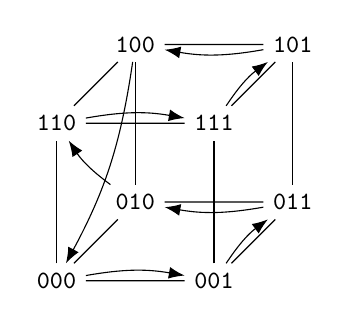
\begin{tikzpicture}[scale=1.0, every node/.style={font=\small}]
    % cube vertices (2D projection)
    \node (A) at (0,0) {\texttt{000}};
    \node (B) at (2,0) {\texttt{001}};
    \node (C) at (3,1) {\texttt{011}};
    \node (D) at (1,1) {\texttt{010}};
    \node (E) at (0,2) {\texttt{110}};
    \node (F) at (2,2) {\texttt{111}};
    \node (G) at (3,3) {\texttt{101}};
    \node (H) at (1,3) {\texttt{100}};

    % cube edges
    \draw (A) -- (B) -- (C) -- (D) -- (A);
    \draw (E) -- (F) -- (G) -- (H) -- (E);
    \draw (A) -- (E);
    \draw (B) -- (F);
    \draw (C) -- (G);
    \draw (D) -- (H);

    % Gray Hamiltonian cycle arrows: 000→001→011→010→110→111→101→100→000
    \draw[-{Latex[length=2mm]}] (A) to[bend left=10] (B);
    \draw[-{Latex[length=2mm]}] (B) to[bend left=10] (C);
    \draw[-{Latex[length=2mm]}] (C) to[bend left=10] (D);
    \draw[-{Latex[length=2mm]}] (D) to[bend left=10] (E);
    \draw[-{Latex[length=2mm]}] (E) to[bend left=10] (F);
    \draw[-{Latex[length=2mm]}] (F) to[bend left=10] (G);
    \draw[-{Latex[length=2mm]}] (G) to[bend left=10] (H);
    \draw[-{Latex[length=2mm]}] (H) to[bend left=10] (A);
  \end{tikzpicture}
  \caption{Minimal Hamiltonian Gray cycle on the 3\,\mbox{\textendash}\,cube \(Q_{3}\): length 8, visits all vertices once, establishes the eight\,\mbox{\textendash}\,tick minimal cadence.}
\end{figure}

\subsection*{Exactness diagram: \(w=\nabla \phi\) (gauge up to constants)}
\begin{figure}[t]
  \centering
  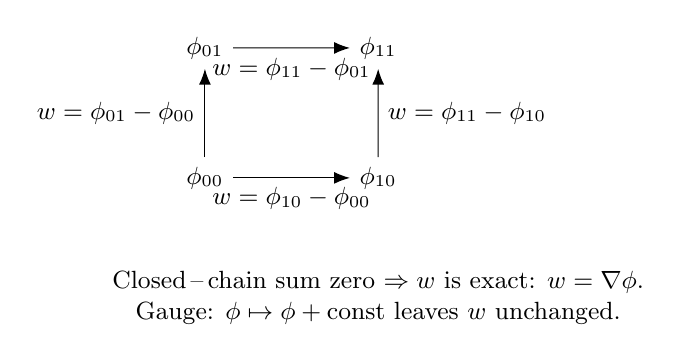
\begin{tikzpicture}[scale=1.1, every node/.style={font=\small}]
    % grid vertices with potential labels
    \node (v00) at (0,0) {$\phi_{00}$};
    \node (v10) at (2,0) {$\phi_{10}$};
    \node (v01) at (0,1.5) {$\phi_{01}$};
    \node (v11) at (2,1.5) {$\phi_{11}$};
    % edges with w labels
    \draw[-{Latex[length=2mm]}] (v00) -- node[below] {$w=\phi_{10}-\phi_{00}$} (v10);
    \draw[-{Latex[length=2mm]}] (v01) -- node[below] {$w=\phi_{11}-\phi_{01}$} (v11);
    \draw[-{Latex[length=2mm]}] (v00) -- node[left] {$w=\phi_{01}-\phi_{00}$} (v01);
    \draw[-{Latex[length=2mm]}] (v10) -- node[right] {$w=\phi_{11}-\phi_{10}$} (v11);
    % closed chain sum annotation
    \node[below=8mm of v10, align=center] (cap) {Closed\,\mbox{\textendash}\,chain sum zero \(\Rightarrow w\) is exact: \(w=\nabla\phi\).\\ Gauge: \(\phi\mapsto\phi+\text{const}\) leaves \(w\) unchanged.};
  \end{tikzpicture}
  \caption{Discrete exactness: edge field \(w\) as a gradient of a node potential \(\phi\), unique up to an additive constant on each component.}
\end{figure}

\subsection*{Identity\,\mbox{\textendash}\,gate schematic and audit table}
\begin{figure}[t]
  \centering
  \begin{tikzpicture}[node distance=16mm, every node/.style={font=\small}]
    \node[draw, rounded corners, padding=2pt] (ell) {$\ell_{0}$};
    \node[draw, rounded corners, right=of ell, padding=2pt] (tau) {$\TauZero$};
    \node[draw, rounded corners, above right=10mm and 10mm of tau, padding=2pt] (c) {$c$};
    \node[draw, rounded corners, below=of tau, padding=2pt] (Ecoh) {$E_{\mathrm{coh}}$};
    \node[draw, rounded corners, right=of Ecoh, padding=2pt] (hbar) {$\hbar$};
    \node[draw, rounded corners, right=22mm of c, padding=2pt] (lambda) {$\lambda$};
    \node[draw, rounded corners, below=of lambda, padding=2pt] (G) {$G$};
    % arrows with identity labels
    \draw[-{Latex[length=2mm]}] (ell) -- node[above] {$c=\ell_{0}/\TauZero$} (c);
    \draw[-{Latex[length=2mm]}] (tau) -- (c);
    \draw[-{Latex[length=2mm]}] (Ecoh) -- node[below] {$\hbar=E_{\mathrm{coh}}\,\TauZero$} (hbar);
    \draw[-{Latex[length=2mm]}] (c) -- node[above] {$\dfrac{c^{3}\,\lambda^{2}}{\hbar\,G}=1$} (lambda);
    \draw[-{Latex[length=2mm]}] (hbar) -- (lambda);
    \draw[-{Latex[length=2mm]}] (G) -- (lambda);
    % alpha box
    \node[draw, rounded corners, above=of lambda, padding=2pt] (alpha) {$\alpha^{-1}=\alpha_{\mathrm{seed}}-w_{8}\ln\phiG-\delta_{\kappa}$};
  \end{tikzpicture}
  \caption{Identity gates among \(c,\,\hbar,\,\lambda,\,G\) with \(\alpha\) pipeline shown separately. Gates enforce invariant ratios; audits require dual\,\mbox{\textendash}\,route agreement within uncertainty bands.}
\end{figure}

\begin{table}[t]
  \centering
  \caption{Audit table for identity gates (classical display; no fit parameters).}
  \vspace{2mm}
  \begin{tabular}{@{} l l l l @{}}
    \toprule
    \textbf{Identity} & \textbf{Form} & \textbf{Inputs} & \textbf{Invariant?} \\
    \midrule
    Speed & $c=\ell_{0}/\TauZero$ & $(\ell_{0},\TauZero)$ & Yes \\
    Coherence & $\hbar=E_{\mathrm{coh}}\,\TauZero$ & $(E_{\mathrm{coh}},\TauZero)$ & Yes \\
    Planck length & $\dfrac{c^{3}\,\lambda^{2}}{\hbar\,G}=1$ & $(c,\,\lambda,\,\hbar,\,G)$ & Yes \\
    Fine\,\mbox{\textendash}\,structure & $\alpha^{-1}=\alpha_{\mathrm{seed}}-w_{8}\ln\phiG-\delta_{\kappa}$ & $(\phiG, w_{8})$ & Yes \\
    \bottomrule
  \end{tabular}
\end{table}

\section{Predictions and tests across scales}

\paragraph{Microscopic.}
Path weights take the exponential form \(w[\gamma]=\exp\big(-\C[\gamma]\big)\). For a discrete alternative set \(\{\gamma_i\}\), operational probabilities follow the normalized weights
\begin{equation}
  P_i \;=\; \frac{\exp\big(-\C[\gamma_i]\big)}{\sum_j \exp\big(-\C[\gamma_j]\big)}\,.
\end{equation}
Permutation symmetry of indistinguishable alternatives yields the standard statistics in the usual way. A practical collapse threshold is set by the recognition action: when the accumulated cost exceeds unity,
\begin{equation}
  \C\;\ge\;1\,,
\end{equation}
definite outcomes (pointers) are observed within the same dynamics (no added postulate). This furnishes a laboratory criterion for onset of classical readout.

\paragraph{Spectral ladders.}
Fixed\,\mbox{\textendash}\,point scaling organizes spectra into \(\phiG\)\,\mbox{\textendash}\,tier families (``rungs''). At a given display scale, ratios become purely geometric:
\begin{equation}
  \frac{X_i}{X_j} \;=\; \phiG^{\,\Delta r}\,,\qquad \Delta r:=r_i-r_j\in\mathbb{Z}\,.
\end{equation}
Predictions are independent of the absolute normalization so long as comparisons are made at the same invariant layer. This yields sharp, scale\,\mbox{\textendash}\,free tests across families.

\paragraph{Large\,\mbox{\textendash}\,scale dynamics.}
On coarse scales, effective weights can be written in a time\,\mbox{\textendash}\,kernel form \(w=w(k,a)\) that depends only on dimensionless combinations (e.g., \(a/(k\,\TauZero)\)), ensuring invariance under admissible unit changes. In weak fields, the mapping acts as a 
purely multiplicative factor on classical sources/observables. For example, for rotational support in a thin disc,
\begin{equation}
  v_{\mathrm{model}}^{2}(r) \;=\; w(r)\,v_{\mathrm{baryon}}^{2}(r)\,,
\end{equation}
with \(w\ge 1\) monotone in the appropriate dimensionless argument. Because \(w\) is fixed by invariants, no per\,\mbox{\textendash}\,object tuning is permitted; predictions can be audited against ensembles with global settings held fixed.

\end{document}


